% IEEE Conference Template for ML/AI Papers
% Document class specification - conference format for IEEE
\documentclass[conference]{IEEEtran}

% Override command lockouts (typically needed for IEEE papers)
\IEEEoverridecommandlockouts
% The preceding line is only needed to identify funding in the first footnote. If that is unneeded, please comment it out.

%%%%%%%%%%%%%%%%%%%%%%%%%%%%%%%%%%%%%%%%%
% PACKAGES
%%%%%%%%%%%%%%%%%%%%%%%%%%%%%%%%%%%%%%%%%
% Citation management
\usepackage{cite}                    % For bibliography citations

% Text and list formatting
\usepackage{enumitem}                % Enhanced list environments
\usepackage{amsmath,amssymb,amsfonts} % Mathematical symbols and fonts

% Algorithms
\usepackage{algorithm}               % For algorithm environments
\usepackage{algorithmic}             % For algorithm formatting

% Graphics and visual elements
\usepackage{graphicx}                % For including images
\usepackage{textcomp}                % Text companion fonts
\usepackage{xcolor}                  % For colored text
\usepackage{forest}                  % For drawing tree diagrams

% TikZ and related packages for diagrams
\usepackage{tikz}                    % Core package for creating graphics
\usepackage{adjustbox}               % For scaling figures
\usepackage{url}                     % For formatting URLs

% Figure and table enhancements
\usepackage{pgfplots}                % For creating plots
\usepackage{booktabs}                % For professional-looking tables
\usepackage{colortbl}                % For colored table cells

% TikZ libraries for specific diagram types
\usetikzlibrary{shapes.geometric,arrows,positioning,fit,backgrounds,calc,decorations.pathreplacing,decorations.markings,patterns,circuits.logic.US,matrix,chains}

% Table enhancements
\usepackage{threeparttable}          % For table notes
\usepackage{cuted}                   % For multi-column environments

% Custom command for line breaks in author block
\makeatletter
\newcommand{\linebreakand}{%
  \end{@IEEEauthorhalign}
  \hfill\mbox{}\par
  \mbox{}\hfill\begin{@IEEEauthorhalign}
}
\makeatother

% Define custom colors for visualizations
% These are common colors used in AI/ML papers
\definecolor{qubitblue}{RGB}{70,130,180}      % Blue for primary elements
\definecolor{controlred}{RGB}{220,20,60}      % Red for control elements
\definecolor{aigreen}{RGB}{50,150,50}         % Green for AI components
\definecolor{quantumpurple}{RGB}{128,0,128}   % Purple for quantum elements
\definecolor{errororange}{RGB}{255,140,0}     % Orange for error highlighting

%%%%%%%%%%%%%%%%%%%%%%%%%%%%%%%%%%%%%%%%%
% DOCUMENT BEGINS
%%%%%%%%%%%%%%%%%%%%%%%%%%%%%%%%%%%%%%%%%
\begin{document}

%%%%%%%%%%%%%%%%%%%%%%%%%%%%%%%%%%%%%%%%%
% TITLE SECTION
%%%%%%%%%%%%%%%%%%%%%%%%%%%%%%%%%%%%%%%%%
\title{[Your Paper Title: Should Be Specific and Descriptive]}

\author{
    \IEEEauthorblockN{
        [Author 1]\textsuperscript{*, a, b},
        [Author 2]\textsuperscript{a},
        [Author 3]\textsuperscript{c}, 
        [Author 4]\textsuperscript{d}
        % Add more authors as needed
    }
    \IEEEauthorblockA{
        \textsuperscript{a}[Institution 1, Country]
    }
    \IEEEauthorblockA{
        \textsuperscript{b}[Institution 2, Country]
    }
    \IEEEauthorblockA{
        \textsuperscript{c}[Institution 3, Country]
    }
    % Add more institutions as needed
    \IEEEauthorblockA{
        *Corresponding Email: [email@example.com]
    }
}

\maketitle

%%%%%%%%%%%%%%%%%%%%%%%%%%%%%%%%%%%%%%%%%
% KEYWORDS
%%%%%%%%%%%%%%%%%%%%%%%%%%%%%%%%%%%%%%%%%
\begin{IEEEkeywords}
[Keyword 1], [Keyword 2], [Keyword 3], [Keyword 4], [Keyword 5]
\end{IEEEkeywords}

%%%%%%%%%%%%%%%%%%%%%%%%%%%%%%%%%%%%%%%%%
% ABSTRACT
%%%%%%%%%%%%%%%%%%%%%%%%%%%%%%%%%%%%%%%%%
\begin{abstract}
[Your abstract should be a single paragraph (150-250 words) that summarizes your work. It should clearly state: 
(1) the problem addressed, 
(2) your approach/methodology, 
(3) key results, and 
(4) main conclusions or implications. 
Be specific and quantitative about your findings. Avoid citations in the abstract.]
\end{abstract}

%%%%%%%%%%%%%%%%%%%%%%%%%%%%%%%%%%%%%%%%%
% INTRODUCTION
%%%%%%%%%%%%%%%%%%%%%%%%%%%%%%%%%%%%%%%%%
\section{Introduction}
[The introduction should:
- Establish the context and importance of your work
- Clearly state the problem or research question
- Briefly review relevant prior work (with citations using \verb|\cite{key}|)
- Outline your approach and contributions
- Provide a roadmap for the rest of the paper

Example citation: Previous work \cite{author2023paper} has shown...]

%%%%%%%%%%%%%%%%%%%%%%%%%%%%%%%%%%%%%%%%%
% RELATED WORK
%%%%%%%%%%%%%%%%%%%%%%%%%%%%%%%%%%%%%%%%%
\section{Related Work}
[This section should:
- Review the most relevant prior work thoroughly
- Group related approaches together
- Highlight limitations of existing methods
- Explain how your work differs from or builds upon previous approaches
- Use citations for all key claims \cite{author2022method}]

%%%%%%%%%%%%%%%%%%%%%%%%%%%%%%%%%%%%%%%%%
% METHODOLOGY
%%%%%%%%%%%%%%%%%%%%%%%%%%%%%%%%%%%%%%%%%
\section{Methodology}
[Describe your approach in detail. This section may include:
- The problem formulation or task definition
- Your proposed method or algorithm
- Technical details and mathematical formulations
- Implementation details
- Example mathematical equation:]

\begin{equation}
    \mathcal{L}(\theta) = \mathbb{E}_{(x,y) \sim \mathcal{D}} [L(f_\theta(x), y)]
\end{equation}

[You can include subsections to organize the content:]

\subsection{Problem Formulation}
[Define the problem formally]

\subsection{Proposed Approach}
[Describe your method]

%%%%%%%%%%%%%%%%%%%%%%%%%%%%%%%%%%%%%%%%%
% FIGURES & DIAGRAMS
%%%%%%%%%%%%%%%%%%%%%%%%%%%%%%%%%%%%%%%%%
% Example figure using TikZ
\begin{figure}[t]
    \centering
    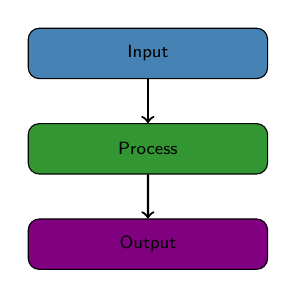
\begin{tikzpicture}[
        scale=0.8, transform shape,
        node distance=0.7cm,
        box/.style={rectangle, rounded corners, draw, fill=#1, text=black, 
            minimum width=3.8cm,
            minimum height=0.8cm,
            align=center, font=\sffamily\footnotesize}
    ]
        % Add TikZ code here for your diagram
        % Example:
        \node[box=qubitblue] (node1) {Input};
        \node[box=aigreen, below=of node1] (node2) {Process};
        \node[box=quantumpurple, below=of node2] (node3) {Output};
        
        % Connections
        \draw[->, thick] (node1) -- (node2);
        \draw[->, thick] (node2) -- (node3);
    \end{tikzpicture}
    \caption{[Caption describing your figure. Be specific and ensure the figure can be understood independently of the main text.]}
    \label{fig:example}
\end{figure}

%%%%%%%%%%%%%%%%%%%%%%%%%%%%%%%%%%%%%%%%%
% EXPERIMENTS
%%%%%%%%%%%%%%%%%%%%%%%%%%%%%%%%%%%%%%%%%
\section{Experiments}
[This section should describe:
- Datasets used
- Evaluation metrics
- Implementation details
- Baseline methods for comparison
- Experimental setup
- Results and analysis]

\subsection{Experimental Setup}
[Describe your datasets, metrics, and implementation details]

\subsection{Results and Analysis}
[Present and analyze your results]

% Example table
\begin{table}[t]
\centering
\caption{[Table caption describing the data presented]}
\label{tab:results}
\begin{tabular}{lccc}
\toprule
\textbf{Method} & \textbf{Metric 1} & \textbf{Metric 2} & \textbf{Metric 3} \\
\midrule
Baseline 1 & 0.XX & 0.XX & 0.XX \\
Baseline 2 & 0.XX & 0.XX & 0.XX \\
Our Method & \textbf{0.XX} & \textbf{0.XX} & \textbf{0.XX} \\
\bottomrule
\end{tabular}
\end{table}

%%%%%%%%%%%%%%%%%%%%%%%%%%%%%%%%%%%%%%%%%
% CONCLUSION
%%%%%%%%%%%%%%%%%%%%%%%%%%%%%%%%%%%%%%%%%
\section{Conclusion}
[Summarize your main findings, contributions, and their implications. Discuss limitations and potential future work.]

%%%%%%%%%%%%%%%%%%%%%%%%%%%%%%%%%%%%%%%%%
% BIBLIOGRAPHY
%%%%%%%%%%%%%%%%%%%%%%%%%%%%%%%%%%%%%%%%%
\bibliographystyle{ieeetr}  
\bibliography{references} % References are in references.bib file

\end{document} 
